\documentclass[10pt,a4paper,twocolumn]{article}
\usepackage{bachelorproject}

\title{Predicting Working Memory Load and Visuospatial Demands During Driving Using Eye-Tracking}

\author{Gilles Lijnzaad, s3409082, m.f.lijnzaad@student.rug.nl}

\supervisors{Dr.\ J.P. Borst \& M. Held, M.Sc.}

\babelhyphenation[english]{spee-do-me-ter}
\newcommand{\nback}{\(n\)-back\ }

\begin{document}

\twocolumn[
  \maketitle
  \begin{@twocolumnfalse}
    % !TEX root = thesis.tex

\begin{abstract}
In adaptive driving, control over the vehicle is dynamically divided between the driver and an intelligent system. 
In order to develop a system that adapts its degree of control to the mental state of the driver, a robust method of measuring their cognitive load is required.
This study focuses on pupillometry as a possible predictor for cognitive load, which is here defined as a combination of working memory load (WML) and visuospatial demands. 
We expected to find a positive correlation between cognitive load and pupil size.
Additionally, we were interested in the effect of cognitive load on speed-keeping efforts, as measured by eye fixations on the speedometer. 
We expected to find a negative correlation between cognitive load and speedometer checking.

To investigate this, a simulated-driving experiment with eye-tracking was conducted in which WML and visuospatial demands were manipulated separately. 
In the simulation participants drove on a straight highway for 60 minutes. 
WML was manipulated by an \(n\)-back task (\(n = 0,1,2,3,4\)), performed by means of speed regulation. 
Visuospatial demands were manipulated by a change in the driving environment: a construction site with reduced lane width, increasing driving difficulty. 

Results indicate that pupil size is a predictor for WML, but not for visuospatial demands. 
We conclude that in order to fully capture cognitive load while driving, pupillometry should be used in combination with a measure of visuospatial demands.
Moreover, a negative correlation between WML and number of fixations on the speedometer was found. 
This highlights speed-keeping aid as an application for adaptive automation based on cognitive load.

\vspace{6ex}
\end{abstract}
  \end{@twocolumnfalse}
]

\thispagestyle{firststyle}

% !TEX root = thesis.tex

\section{Introduction}\label{sec:introduction}

% ----- GENERAL EXPLANATIONS -----
% driving
Driving a car is a challenging task. 
It involves processing a large number of stimuli and constantly updating a mental model of the environment.
Not to mention, operating a vehicle requires making appropriate decisions to ensure the safety of both the driver and other road users.
Driving is even more challenging for young and novice drivers. 
They are more prone to a high level of mental workload than experienced drivers due to their low level of operating skills, lack of driving experience \citep{Gregersen1996} and not fully-matured prefrontal cortex \citep{Ross2014}.
This in turn is one of the causes for the relatively large number of traffic accidents that young drivers are involved in \citep{Sena2013}.
And indeed, more generally, human failure is the cause of the majority of traffic accidents \citep{DeWaard1996}.

% automated driving
An often proposed solution to this issue is automated driving, which refers to the vehicle being operated by an intelligent system \citep{Cabrall2018}.
However, \citet{Brookhuis2007} state that human supervision is necessary even in fully automated driving to handle abnormal situations.
Situations where the human operator must suddenly take back manual control then pose a serious risk.
The driver is likely to respond inadequately due to their reduced attentional awareness and the erosion of their operating skills \citep{Dijksterhuis2012}.
This is where adaptive automation comes into play.

% adaptive automation
In adaptive automation the division of control between the machine and the human operator is not static.
Rather, it is based on changes in the physical environment or the condition of the operator \citep{Sheridan2011}.
An important facet of this is adaptive automation based on the human factor of mental workload.
An intelligent car that counteracts the negative effects of a high cognitive load on driving performance can greatly benefit the driver's safety.

% cognitive load
We must first ask what the concept of cognitive load means.
Let us define cognitive load as the level of perceived cognitive effort when performing a task.
Two elements to cognitive load are most important in the context of driving: \textit{central} and \textit{visual} demands \citep{DeWaard1996}. 

% explain WML as factor to cognitive load
Central demands have to do with working memory load (WML).
In driving, working memory plays an important role in remaining focused on the task at hand; in other words, maintaining cognitive control \citep{Wood2016}.
It is also important in maintaining task goals, whether high-level (for example, planning a route) or low-level (for example, planning an overtaking manoeuvre).

% explain visuospatial demands factor to cognitive load
The task of driving has some intricate visual demands as well.
Visuospatial attention is required to process the movement of objects in traffic such as cars, pedestrians and traffic signs \citep{Zheng2020}.
This is a reflected by a number of studies on road accidents, linking reduced visuospatial attentional abilities --due to for example old age-- to deteriorating driving performance (for a review see \citealp{Owsley2010}).
In practice, the requirement of visuospatial attention means that drivers must continuously scan their environment since criticial visual events can occur anywhere at any time.

% cognitive load + pupil size: RQ and hypothesis
In order to develop a system that adapts to the driver's cognitive load it is essential to find a robust method of measuring cognitive load.
Changes in an individual's cognitive load are reflected by a number of physiological measures including heart rate variability, brainwave levels (as measured by an electroencephalogram; EEG), skin galvanic response and pupillary response \citep{Haapalainen2010}.
The current study focuses on the latter as a predictor for cognitive load. We attempt to find whether the current level of cognitive load, defined as a combination of working memory load and visuospatial demands, can be predicted by pupil size.

Following results by \citet{Palinko2010} we expect that pupillometry can provide a viable estimation for cognitive load while driving. 
Furthermore, results by \citet{Scheunemann2019} suggest an interaction between central and visual demands during driving at the brain level.
This interaction effect between the two components of cognitive load is expected to be reflected in pupil size.

% cognitive load + speed-keeping: RQ and hypothesis
Additionally, we are interested in the effect of cognitive load on speed-keeping.
A relationship between cognitive load and speed-keeping performance would reveal that speed-keeping is a necessary application of adaptive automation. 
That is, if a high cognitive load leads to diminished speed-keeping performance, then adaptive automation should aid the driver with keeping their speed when under high load.
In this study we will use eye fixations on the speedometer as a measure of speed-keeping efforts. We therefore ask whether the number of eye fixations on the speedometer correlates with the current level of cognitive load.

Based on the notion of limited cognitive resources (as described by \citet{DeWaard1996}) we expect there to be negative correlation between cognitive load and fixations on the speedometer.
As an example consider an easy driving task which requires little cognitive resources to be spent.
This then leaves plenty of cognitive resources for checking the speedometer.
In contrast, a driving task with high visuospatial or central demands allows little ``mental space'' to concern oneself with the speedometer.
Findings by \citet{Salvucci2011} support this claim, suggesting that drivers perform less control updates (such as checking the speedometer) when engaging in a demanding secondary task.

% OPERATIONALISATION
In order to test these two hypotheses a simulated-driving experiment with eye-tracking was conducted in which central and visual demands were manipulated separately.
It largely follows the approach of \citet{Scheunemann2019} who studied the interaction between working memory load (WML) and visuospatial demands while driving.
Their experiment involved participants driving a car on a highway in a realistic simulation. 

% working memory load
WML was manipulated through an \nback task, which is considered to be a standard measure of working memory in cognitive neuroscience \citep{Kane2007}.
The task was integrated into the driving process by means of speed regulation, meaning participants were instructed to drive according to the speed sign that occurred \(n\) signs ago.

% visuospatial demands
Visuospatial demands were manipulated by contrasting two driving environments: \textit{construction} and \textit{non-construction}.
In the non-construction condition participants drove on a regular three-lane highway.
In the construction condition the leftmost lane was closed off by a continuous row of pylons and the remaining two lanes were of reduced width, which increases driving difficulty \citep{Liu2016}.
% !TEX root = thesis.tex

\section{Methods}\label{sec:methods}
Following~\cite{Unni2017} an \(n\)-back task with five levels (\(n = 0,1,2,3,4\)) was used to manipulate working memory load. 
This task was integrated into the driving task by means of speed regulation. 
The designed environment also had an additional working memory constraint: a construction site with narrower lanes.  

\subsection{Participants}
A total of 38 volunteers (23 male, 12 female, 3 other) aged 20--36 (\(M = 23.1 \pm 3.0\)), possessing a category B driver's license, participated in this experiment. 
All participants signed an informed consent form prior to the experiment and were compensated 12 euros for their participation.

\subsection{Experimental Set-up}
The experiment took place on a simulated three-lane highway with no major turns/bends in the road. 
The features of the environment were minimal. 
Either side of the road was coloured green, signifying grass. 
There were no median strips dividing the road from the rest of the environment. 
Apart from a single other car, represented by a blue rectangle and referred to as the \textit{autocar}, there were no other objects/traffic on the highway. 
The autocar would stick to traffic rules such as overtaking from the left, staying on the right lane as much as possible, and following the current speed limit. 

The participant could see a black dashboard that filled the bottom of the screen. 
Here the speed of the car was visible (as an integer). 
When the left or right indicators were pressed, they would appear on the dashboard in the respective sides as yellow blinking arrows. 
The simulation had three rear-view mirrors: one on the top, one on the left, and one on the right. 
The autocar was visible in the corresponding mirrors depending on the distance from the car. 

In the construction condition the leftmost lane is closed off by a continuous row of pylons. 
The lanes were separated by a full yellow line and were narrower than the non-construction condition. 

Speed signs that passed were identical to general speed signs in The Netherlands; black digits enclosed by a red circle. 

% explain n-back task
Within each trial the participants were presented with at least nine speed signs at intervals of 20 seconds, with the exception of the first speed sign appearing after 5 seconds. 
For \(n\)-back tasks with \(n > 0\), there was a build-up phase of \(n\) speed signs preceding the nine speed signs where the participant would perform the task. 
For example, for \(n = 4\), the build-up phase would be the first four speed signs. 
After the build-up phase, the task of regulating speed would start. 
Due to a difference in length of build-up phases per \(n\)-back trial, each trial differs in number of speed signs, as well time taken.

% equipment and stuff
Participants interacted with the simulation using a steering wheel with blinkers and a throttle and brake pedal (Driving Force GT by Logitech). 
The steering wheel was secured to the table in front of the screen and remained in the same location for all participants. 
The pedals were placed on the floor such that participants could move it closer or further depending on their level of comfort. 
An eye-tracking camera (EyeLink Portable Duo, SR Research, Missisauga, Canada), placed between the screen and the steering wheel, was used to continuously record the eye movements and pupil size of participants. 

\subsection{Experimental Procedure}
The procedure of the current experiment follows that of \citet{Scheunemann2019}.
The experiment consisted of 20 trials in total, divided by a short break into two blocks of 10 trials each. 
Within a block, each \(n\)-back trial appeared twice: once with a construction site and once without. 
The order of the trials was determined pseudorandomly with a few conditions. 
Firstly, no \(n\)-back level could appear twice in a row. 
Secondly, the construction/non-construction conditions were alternated from trial to trial. 
These constraints on the randomization were incorporated with the aim of avoiding habituation effects for the memory task and the visuospatial demands. 
Finally, the order of the trials in the first block was reversed to form the order of trials in the second block.

Prior to performing the experiment the participant was given instructions about the driving and the memory task. 
They then performed a practice round (one 2-back trial with no construction and a total of 5 speed signs) to get accustomed to the simulation and the steering wheel. 
Next, the eye-tracker was calibrated. 
This involved the participant following a target around the computer screen with their eyes. 
This procedure was repeated twice: once to calibrate and once to validate whether that calibration was accurate. 
Calibration was performed again in the case that the validation was inaccurate.

After calibration, the experiment began. 
Before every trial a pop-up message appeared telling the participant which \(n\)-back task they should perform in the next trial. 
The percentage of total trials they had already completed was also shown in the message. 
Furthermore, every trial (excluding the very first one) was preceded by an eye-tracking drift correction. 
This required the participant to look at a target at the center of the screen. 
If the measured eye position deviated too far from the position of the target, calibration was performed again. 
Otherwise the deviation was automatically taken into account with recording of the eye position. 

\subsection{Data collection}
A number of different variables pertaining to driving behavior were recorded at a rate of 200 Hz. 
The use of the accelerator and brake pedals was recorded as numbers ranging from 0 (not pressed) to 1 (fully pressed). 
The angle of the steering wheel was recorded as a number ranging from -1 (left) to 1 (right).
In order to measure lane centering, the position and orientation of the participant's car were recorded as [measure]. 
Finally, the speed of the participant's car was recorded along with the occurring speed signs to calculate \(n\)-back task performance. 

The eye-tracker recorded a number of raw variables at a rate of 500 Hz, two of which are relevant for the current study.
Eye positions are measured in \(x\) and \(y\) coordinates relative to the PC monitor (\(1920 \times 1080\) px).
Pupil size was measured in terms of diameter in arbitrary units. 

\subsection{Data analysis}
The raw eye-tracking data were sorted into fixations, saccades and blinks using the \texttt{eyelinker} R package\footnote{\url{https://CRAN.R-project.org/package=eyelinker}}.
Only the fixations were used for data analysis as this eliminated a lot of noise and reduced the amount of data by around 99\%, making it much more workable.
For both variables of interest discussed in the introduction (pupil size and fixations on the speedometer) some preprocessing was required.

To properly compare pupil size, baseline correction is required. 
According to \citet{Mathot2018} baseline correction increases statistical power by accounting for random fluctuations in pupil size over the course of an experiment.
To this end the baseline pupil size is recalculated for each new trial.
As a baseline period we chose the time period between the start of the trial and the appearance of the first speed sign.
The mean pupil size during this 5 second interval was used to correct the pupil sizes of the trial.
More specifically we have chosen to use subtractive baseline correction (\(corrected\ pupil\ size = pupil\ size - baseline\)) 
as \citet{Mathot2018} prefer it over divisive baseline correction (\(corrected\ pupil\ size = pupil\ size / baseline\)).

The analysis of fixations on the speedometer required some preprocessing as well.
On the surface it seems fairly simple to define the speedometer as an area of interest (AOI) and count the number of fixations within that area.
Yet, shifts in eye positions between and within participants made it impossible to universally define the bounds of this AOI.\@
For this reason we manually determined the borders of the AOI for each participant, i.e.\ determined what ``counts as'' a fixation on the speedometer.
Fixations on the speedometer will be expressed as a percentage of the total number of fixations during that trial to account for [reason].

We will focus on three measures relating to the two variables of interest. 
Pupil size will be examined both between and within trials.
These two temporal contexts will provide a detailed image of how a participant's pupil size changes over time.
Fixations on the speedometer will be examined between trials. 
In order to test the significance of the results we will use an ANOVA with repeated measures.

A number of participants was excluded from data analysis.
5 participants were excluded from the entire experiment because their driving behavior was not indicative of an actual attempt to perform the task.
This was determined by their task error on the 0-back, which we expect to be close to zero.
Therefore task error (see \citet{DeMooij2021}) was determined for 33 participants.
For eye-tracking analysis 8 more participants were excluded as their data were either non-existent or incomplete.
This leaves us with 25 participants for eye-tracking analysis.
Finally, for the analysis of lane deviation (see \citet{Kelapanda2021}) 15 participants were excluded because of missing data, leaving 18 participants for analysis.
% !TEX root = thesis.tex

\section{Results}\label{sec:results}
\subsection{Driving behavior}
Figures~? (from \citet{DeMooij2021}) and~? (from \citet{Kelapanda2021}) show behavioral results.
[Explanation of what we see in their plots.]

\subsection{Pupil size}
\begin{figure}[tp]
  \centering
  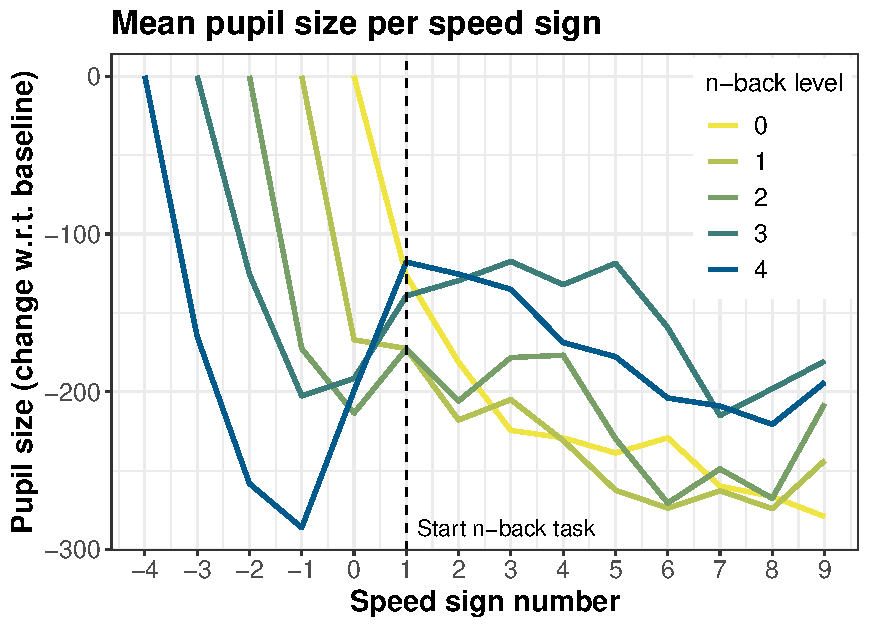
\includegraphics[width=7.5cm]{images/speed_sign_nback.pdf}
  \caption{Mean pupil size over the period between the appearance of two speed signs.
  The dashed vertical line indicates the moment that participants need to start performing the \(n\)-back task by regulating their speed according to the speed signs.
  Pupil size was corrected using subtractive baseline correction and is shown in arbitrary units. 
  The data were smoothed using the loess method.}
  \label{fig:ps-speed-sign}
\end{figure}

Figure~\ref{fig:ps-speed-sign} shows how the pupil size of participants changed within a trial.
There is a visible distinction between change in pupil size for low \(n\)-back levels (\(n = 0,1,2\)) and high \(n\)-back levels (\(n = 3,4\)):
whereas high \(n\)-back levels show a peak in pupil size, low \(n\)-back levels show a decline from the start of the task.
This difference, which can be characterized as an interaction between \(n\)-back level and speed sign number on pupil size, is significant according to an ANOVA with repeated measures [\(F(4,2536)=7.42,\ p < .001\)].
Interestingly, compared to \(n = 3\) the peak in pupil size for \(n = 4\) is higher but shows a sharper decline afterwards.
An explanation for this could be that participants focus their attention on the task at first which causes their pupil to dilate, but then quickly abandon the task because of its difficulty, resulting in a contraction of the pupil.
This theory is supported by the increase in task error for the higher \(n\)-back levels as shown in Figure~?.

\begin{figure}[tp]
  \centering
  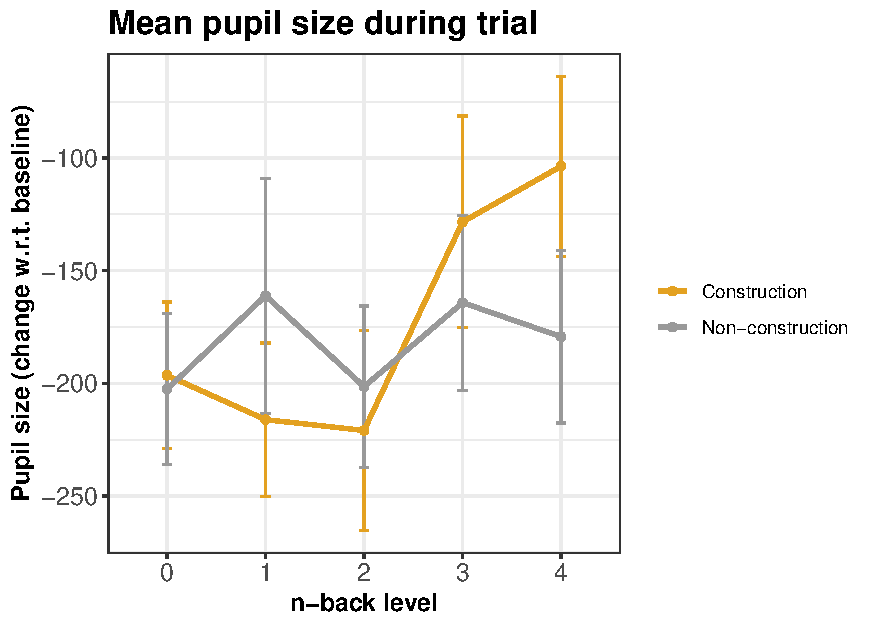
\includegraphics[width=7.5cm]{images/pupil_size_interaction.pdf}
  \caption{Mean pupil size during trial; bars represent standard error.
  Pupil size was corrected using subtractive baseline correction and is shown in arbitrary units.}
  \label{fig:mean-ps}
\end{figure}

Figure~\ref{fig:mean-ps} shows the mean pupil size over an entire trial. 
It suggests that there is no effect of \(n\)-back on pupil size within the non-construction trials.
For the construction trials there seems to be an increase of pupil size by \(n\)-back level more so than for non-construction trials.
However, this suggested interaction between \(n\)-back level and construction on pupil size is not significant [\(F(4,216)=1.50,\ p=.20\)].
Disregarding the difference between construction and non-construction we do find a marginally significant effect of \(n\)-back level on pupil size [\(F(4,221)=2.39,\ p=.052\)].

\subsection{Fixations on speedometer}

\begin{figure}[tp]
  \centering
  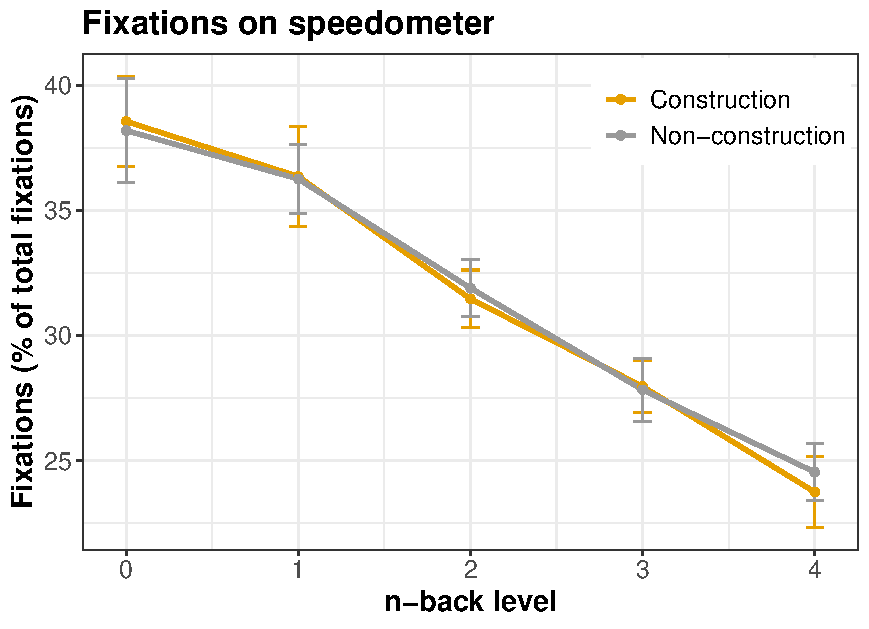
\includegraphics[width=7.5cm]{images/speedometer_interaction.pdf}
  \caption{Number of fixations on the speedometer as a percentage of the total number of fixations for that trial; bars represent standard error.}
  \label{fig:fix-speedometer}
\end{figure}

Figure~\ref{fig:fix-speedometer} shows the number of fixations on the speedometer as a percentage of the total number of fixations for a trial.
Like this figure suggests, there is a significant negative correlation between \(n\)-back level and fixations on the speedometer [\(F(4,221)=84.72,\ p<.001\)] and no effect of construction or an interaction between \(n\)-back and construction. 
% !TEX root = thesis.tex

\section{Discussion}\label{sec:discussion}
In this study we sought to answer two questions related to cognitive load while driving by means of an eye-tracking experiment.
Firstly, can the current level of cognitive load be predicted by pupil size? 
And secondly, does the frequency of fixations on the speedometer correlate with the current level of cognitive load?
Below you will find our conclusions based on the results of the experiment.

Let us first consider the effect of working memory load (WML) on pupil size.
Within trials we found a significant effect of WML and speed sign number on pupil size (see Figure~\ref{fig:ps-speed-sign}).
Most notably we see a contrast between pupil size for low \nback levels (\(n = 0,1,2\)) and high \nback levels (\(n = 3,4\)). 
This contrast between low- and high-level \nback levels is also reflected in task error (see Figure~?, Milan's task error plot). 

Interestingly, compared to \(n = 3\) the peak in pupil size for \(n = 4\) is higher but shows a sharper decline afterwards.
An explanation for this could be that participants focus their attention on the task at first (causing their pupil to dilate), but then quickly abandon the task because of its difficulty, resulting in a contraction of the pupil.

Between trials we also found a significant effect of WML on pupil size. 
We therefore conclude that pupil size is a predictor for WML.\@

However, the same cannot be said for visuospatial demands. No effect of construction condition on pupil size was found, and the expected interaction between WML and visuospatial demands on pupil size was not significant.
Our results therefore suggest that visuospatial demands have little influence on pupil size.
One could take this to mean that changes in pupil size \textit{only} reflect working memory load.

Finally, results showed that the amount of fixations on the speedometer decreases linearly by WML.\@
We conclude that as WML increases, fewer cognitive resources are available for performing control updates.
This could indicate that high WML leads to decreasing speed-keeping efforts.
In this context we again see little to no influence of visuospatial demands, suggesting that only WML affects speed-keeping efforts.

What are then the practical implications of these results? 
We have established that pupillometry can be used to assess working memory load (WML) during driving, yet reveals little about visuospatial demands on the driver.
Since a robust measure of cognitive load must embody both central \textit{and} visual demands, our results challenge the utility of pupillometry in the estimation of drivers' cognitive load.
Further research on the relation between visuospatial demands and pupil size during driving is therefore necessary.
If our findings are further consolidated, pupil size should no longer be a variable of interest in the development of adaptive driving based on cognitive load.

Moreover, the confirmed correlation between WML and speed-keeping efforts highlights speed-keeping as a topic of interest in the field of adaptive automation.
It is important to then first investigate the relationship between speed-keeping efforts and actual performance.

There are some limitations to this study. 
Firstly, for 10 of the 38 participants, trials were shorter than they should have been due to an error in the simulation program.
More specifically, only 9 speed signs were shown for all trials. 
This is the correct number of signs for only the 0-back task.
For all other \nback levels there were \(n\) signs too little. 
This is especially important for the 4-back, where the time spent performing the speed regulation task is essentially halved.
These 10 participants only performed 82\% of the entire experiment.
This problem diminishes the statistical power of our results somewhat.

[I cannot think of any more limitations. Maybe we can discuss it in our meeting this Tuesday.]
% % !TEX root = thesis.tex

\section*{Acknowledgements}\label{sec:acknowledgements}
I would like to thank Jelmer Borst and Moritz Held for their wonderful supervision.
They were readily available for questions and guidance, which I am very appreciative of.

\bibliographystyle{apacite}
\bibliography{literature}

\end{document}
